\section{TRUST EVALUATION METRICS BASED ON THE SUPPORTED PRIVACY LEVEL}
\label{sec:geolocation}
%Description of the OBD system, how data can be retrieved from the car.
Another form of verification is the use of sensors on multiple devices~\cite{ju2012neteye}.  For example,
a smartphone may communicate directly with a smartwatch or on-board diagnostics (OBD)
sensor on an automobile.  These other devices have sensor with the same
functionality as some of the sensors on the smartphone.
% describe what data is collected, how it is stored, and how it might be used.
% we can include a graph of spped error vs time and the picture of the car route
We introduce a case where smartphones communicate with an in-vehicle OBD sensor
to get geolocation information, such as speed, engine RPM, fuel consumption, 
etc.

\subsection{Vehicle data collection}

Our vehicular data collection consists of a process on a mobile 
device that directly communicates with in-vehicle sensors and collects sensor 
data~\cite{sensor}. Data can be encrypted and transferred to our 
centralized server for permanent data storage. \weiss{we should put a diagram of 
the data collection and storage}
To deploy such a process on a mobile device, a device owner first installs an
app~\cite{sensor-app} on their devices\footnote{Currently, Android smartphones 
and tablets are supported.}. Since we are interested in
vehicular data, the target group of device owners are also vehicle 
owners. These owners simply insert their WiFi On-Board Diagnostics 
(OBD)~\cite{obd} sensor into their cars' OBD ports (located under the steering wheel),  
%\linda{I don't think they insert their sensor into the car. Do they insert it into something specific in the car (e.g., a usb port)? That would make sense. Anyway, I think you need to be more specific in stating what gets connected to what} 
and connect their 
smartphone or tablet to the sensor, which also runs as a WiFi access 
point. Note that OBD systems are in most cars and light trucks 
on the road today~\cite{obdconnector}. Therefore, our 
infrastructure does not require extra installation of specialized  
hardware or equipment~\cite{reininger2015first}. 

A person interested in getting vehicular data uploads his  
code to run in the background of the mobile device, and to communicate 
with an in-vehicle OBD sensor to get vehicle data. Device owners need not worry about having to
interact with the app or about being interrupted as they use their smartphones. 
Note that all code runs in a secure sandbox in our 
app~\cite{sensor-app}, which limits the amount of storage, network, 
memory, battery, and CPU resources used by any code~\cite{Cappos_CCS_10}. 
To protect end users' devices from malicious attackers, the sandboxed 
code is securely isolated from other programs on the same device.
Any bugs in the code will be contained in the sandbox, and will not 
affect the rest of the user device~\cite{Cappos_CCS_10}. 
%Once our prototype data collection application is installed and running on an Android smartphone with Sensibility, the end user need not worry about interacting with a user interface on the Android. Rather, once the user inserts their WiFi OBD sensor into the car and connects their Android smartphone to the sensor running as a wifi access point, our 
%

At the remote server, the vehicular sensor data collected from 
multiple end user devices is stored in a non-relational database. 
An example of 
collected data is shown in Figure~\ref{fig:json}, in JSON format.
The collected data set can be visualized on Google Maps to 
identify fuel efficient routes, routes with higher traffic activity, and routes 
(and drivers) that exhibit a high frequency 
of reckless or illegal driving behaviors, etc. 

\begin{figure}
\scriptsize 
\begin{Verbatim}
\{
  \textbf{"sensors"}: \{
    \textbf{"speed_car"}: \textcolor{red}{60},
    \textbf{"maf_car"}: \textcolor{red}{4},
    \textbf{"rpm_car"}: \textcolor{red}{114},
    \textbf{"gps_phone"}: \{
      \textbf{"error"}: \textcolor{red}{null},
      \textbf{"id"}: \textcolor{red}{0},
      \textbf{"result"}: \{
        \textbf{"network"}: \{
          \textbf{"time"}: \textcolor{red}{1407200660927},
          \textbf{"speed"}: \textcolor{red}{60},    
          \textbf{"altitude"}: \textcolor{red}{4.099999904632568},
          \textbf{"bearing"}: \textcolor{red}{82.6999694824219},
          \textbf{"provider"}: \textcolor{OliveGreen}{"gps"},
          \textbf{"longitude"}: \textcolor{red}{-73.986706},
          \textbf{"latitude"}:\textcolor{red}{40.694010},
          \textbf{"accuracy"}: \textcolor{red}{7},
        \}
      \}
    \},
    \textbf{"id"}: \textcolor{OliveGreen}{"310410696731709"},
    \textbf{"time"}: \textcolor{SkyBlue}{"ISODate"}(\textcolor{OliveGreen}{"2014-08-05T21:04:07.183-04:00"})
\}
\end{Verbatim}
\caption{JSON document of vehicular data.\label{fig:json}}
\end{figure}

\subsection{Data store}
Given the variety of sensors on a smartphone,
sensor measurements come in different forms. 
As shown in Figure~\ref{fig:json}, many types of sensor data have complex structure.
As a result, we decided to use a non-relational database, 
MongoDB~\cite{mongodb}, for storing sensor data. MongoDB has a Binary 
JSON (BSON) document-style structure identical to that shown previously 
in Figure~\ref{fig:json}, albeit converted into binary as its name suggests. 
This provides the scalability that is crucial to our system and that allows dynamic storage of 
new sensors, as needed. 

\subsection{Geolocation data analysis}

\begin{table}
\scriptsize
\centering
\begin{tabular}{|p{.06\columnwidth}|p{.18\columnwidth}|p{.22\columnwidth}|p{.28\columnwidth}|}
\cline{2-4}

%\multirow{3}{*}{Statistics}

\multicolumn{1}{c|}{}  & \textbf{GPS speed} & \textbf{Vehicle speed} & \textbf{Speed difference}  \\ \hline

% Mean & 5.559 & 1.568 & 0.003606 \\ \hline 

Med & 53.0~kph & 54.9~kph & 2.15~kph \\ \hline

STD & 12.79~kph & 13.61~kph & 4.57~kph  \\ \hline

\end{tabular}
\caption{\small Speed comparison: GPS speed comparing to OBD speed.}
\label{tab:speed-diff}
%\vspace*{-15pt}
\end{table}

\begin{figure}
\centering
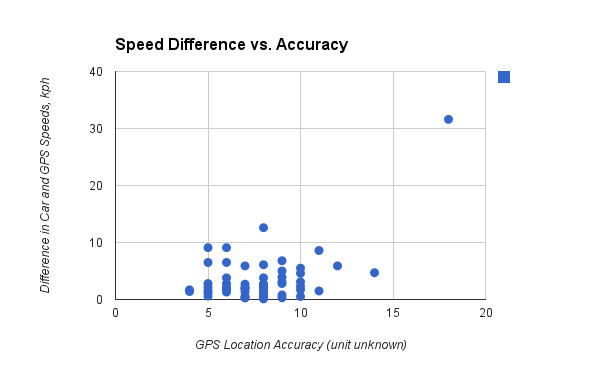
\includegraphics[width=3.5in]{speed.png}
\caption{Speed difference and accuracy.}
\label{fig:speed-diff}
\end{figure}

Using the aforementioned measurement, we collected speed data from both GPS 
on the smartphone inside a vehicle, and the speed via the OBD sensor. 
The data from these two sources can corroborate to verify normal or abnormal 
geolocation data. Table~\ref{tab:speed-diff} shows the median and standard deviation
of the speed measured by GPS and OBD sensor, over 58 data samples collected. 
The overall statistics do not show any anomaly in speed. However, when plotting 
individual data samples, we can see a data outlier in Figure~\ref{fig:speed-diff}. 
Excluding this point, the rest of the data samples roughly follow a Gaussian 
distribution. This outlier seems to be due to the initialization of the
GPS sensor.  Initially, the GPS measurements are underconstrained leading to a large 
geolocation error, which is rapidly reduced as more measurements are made.


\begin{figure}
\centering
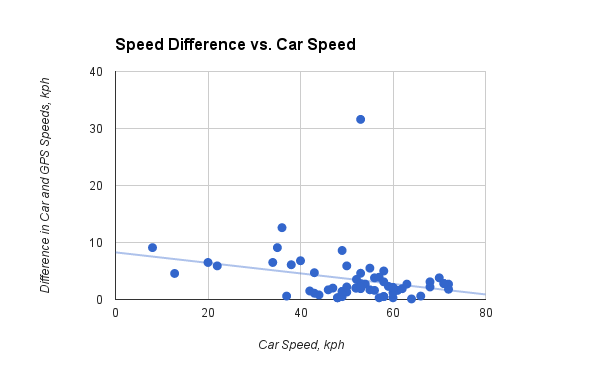
\includegraphics[width=3.5in]{car.png}
\caption{A typical session in Traceview, the execution log viewer.}
\label{fig:car}
\end{figure}

To further investigate on the speed data, we plot the differences between 
vehicle speed and GPS speed, and compare the differences against 
the varying vehicle speed. As shown in Figure~\ref{fig:car}, the speed 
differences are in a linear relation with the vehicle speed 
(other than the outlier), i.e., the 
higher the vehicle speed, the smaller difference between vehicle 
speed and GPS speed. \yanyan{any other observations?} 
The linear relationship in the figure is based on minimum mean 
square error (MMSE) xxx. \yanyan{please fix this}

\begin{figure}
\centering
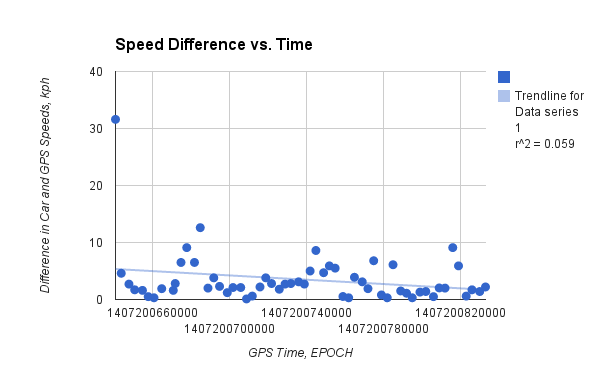
\includegraphics[width=3.5in]{time.png}
\caption{A typical session in Traceview, the execution log viewer.}
\label{fig:time}
\end{figure}

We also investigate the speed differences over time. 
In Figure~\ref{fig:time}, we can conclude that excluding the outlier, 
the differences between 
vehicle speed and GPS speed fluctuate around a constant value over 
time. 
